% !TEX encoding = UTF-8 Unicode
\documentclass[a4paper]{article}

\usepackage[utf8]{inputenc}
\usepackage[francais]{babel}
\usepackage[nonewpage]{imakeidx}
\usepackage{hyperref}
\usepackage{enumitem}
\usepackage{graphicx}

% Glossaire:
\usepackage[acronym,toc,nopostdot]{glossaries}
% !TEX encoding = UTF-8 Unicode
% Glossaire
\newglossaryentry{joueur}
{
    name=joueur,
    description={Personnage fictif du jeux pouvant faire partie d'une équipe et jouant au quiditch.}
}
\newglossaryentry{equipe}
{
    name=équipe,
    description={Elle est composée de 7 \glspl{joueur} (un gardien, un attrapeur, deux batteurs et trois poursuive).}
}
\newglossaryentry{manager}
{
    name=manager,
    description={\Gls{utilisateur} du programme, il possède un \gls{club} et dois faire en sorte que celui-ci gagne de l'argent.}
}
\newglossaryentry{club}
{
    name=club,
    description={Infrastructure contenant une \gls{equipe} et des installations (stade, infirmerie,\ldots).}
}

\newglossaryentry{utilisateur}
{
    name=utilisateur,
    description={Personnage réel. C'est la personne qui joue au Quiditch manager.\\
    Elle est appelée en jeu \gls{manager}}
}

\newglossaryentry{enchere}
{
    name=enchère,
    description={Système permettant l'achat de \glspl{joueur}}
}
\newglossaryentry{serveur}
{
    name=serveur,
    description={Programme étant toujours en marche et connecté à internet et qui réceptionne les connections des \glspl{client}. Il a les données de tous les \glspl{utilisateur}.}
}
\newglossaryentry{client}
{
    name=client,
    description={Programme que l'\gls{utilisateur} lance pour se connecter au \gls{serveur}. Il permet à l'\gls{utilisateur} de jouer et peut être soit en ligne de commande, soit en mode graphique.}
}
\newglossaryentry{participant}
{
    name=participant,
    description={Nom donné à l'\gls{utilisateur} lors d'un tournoi.}
}


% Acronymes

\makeglossaries
\setglossarysection{subsection}
\deftranslation{Glossary}{Glossaire}
\renewcommand*{\glossaryname}{Glossaire}
\DeclareRobustCommand{\gloss}[1]{\it{#1}\index{\glslabel}}
\renewcommand{\glsdisplay}[4]{\gloss{#1#4}}
\renewcommand{\glsdisplayfirst}[4]{\gloss{#1#4}}


\makeindex
\indexsetup{level=\section}
\setcounter{secnumdepth}{4}

\title{Quiddich live : \\Software requirements document}
\author{Bruno Rocha Pereira \and Jérome Vial \and Cédric Strebelle \and
Romain Fontaine \and Tsotne Shonia \and Nikita Marchant}
\date{\today}

% Début du document
\begin{document}

\maketitle

\section{Introduction}
\subsection{But du projet}
Le développement de cette application se fait dans le cadre du projet d'année de BA2 en sciences informatiques à l'Université Libre de Bruxelles. Il consiste en l'implémentation d'un jeu de Quidditch, sport tiré de la saga Harry Potter de J.K.Rowling. 
Le quidditch est un sport pratiqué par deux équipes de 7 joueurs évoluant à l'aide de leur balais sur un terrain de forme ovale. Le but de ces 2 équipes est de marquer le plus de point possible grâce au Souaffles et d'attraper le Vif d'or\footnote{Pour pmlus d'informations, se référer au livre J. K. Rowling, Le Quidditch à travers les âges, Gallimard,‎ 2001.}. 
Le jeu est de type gestion et stratégie en ligne. L'\gls{utilisateur} est le manager d'un club de Quidditch, et son but est de faire progresser son club vers le succès. Pour ce faire, il devra gérer tous les aspects du club, tant au niveau sportif que financier. La saison de Quidditch se déroule sous la forme d'un championnat, durant lequel tous les \glspl{utilisateur} s'affrontent entre eux au cours de matches aussi spectaculaires que tactiques. Les matches seront planifiés dans un calendrier qu'il faudra respecter sous peine de sanction. Un match se joue au tour part tour, mais les deux \glspl{utilisateur} jouent simultanément. Il y a donc une notion importante d'anticipation dans la maîtrise de ce jeu. En ce qui concerne la gestion du club, L'\gls{utilisateur} aura la possibilité de recruter de nouveaux joueurs de Quidditch pour renforcer son équipe, il pourra aussi développer différentes infrastructures et services, comme son stade, son infirmerie, son terrain d'entraînement, son fanshop etc.

% glossaire
\printglossary[numberedsection]
\subsection{Historique}

\section{Besoins d'utilisation}
\subsection{Exigences fonctionnelles}

\subsubsection{Identification}
\paragraph{Inscription}
\begin{figure}[h]
   \caption{\label{1} Inscription}
   \begin{center}
   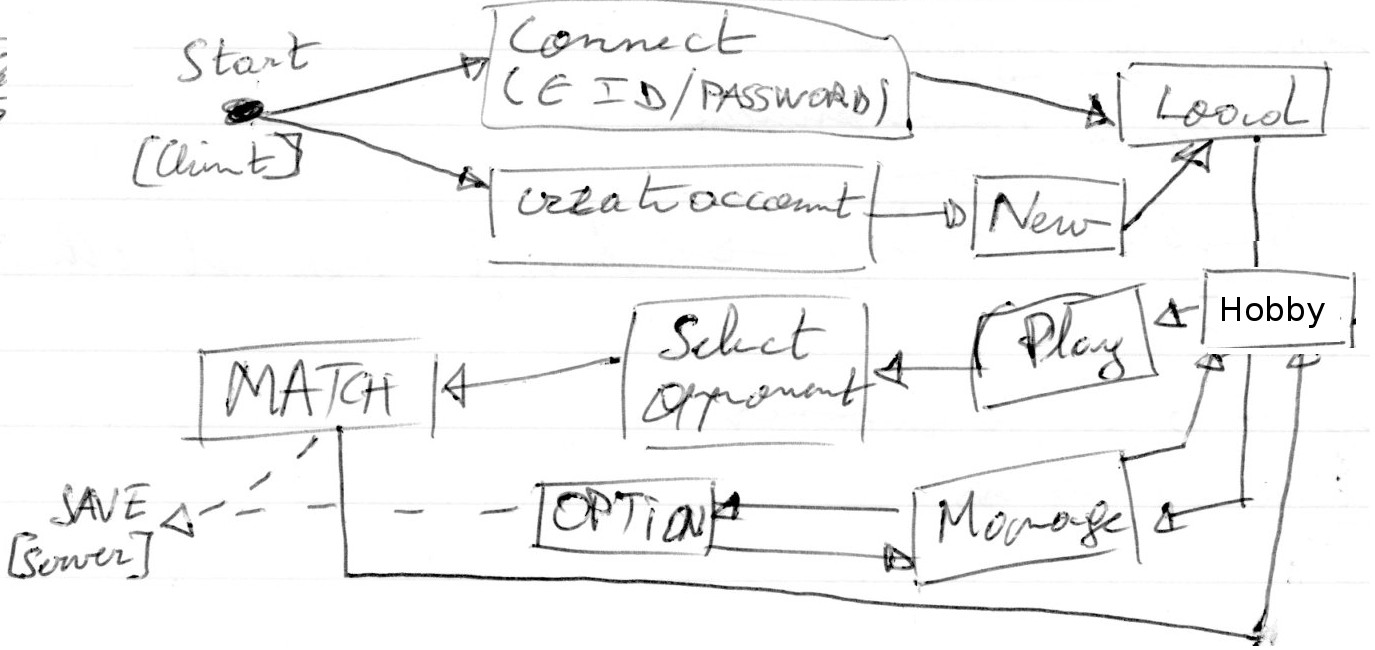
\includegraphics[height=100pt]{../pv/pv1/schema1_pv1.jpg}
   \end{center}
\end{figure}
\begin{description}
\item[Action] L'\gls{utilisateur} doit pouvoir s'inscrire (s'enregistrer) sur le \gls{serveur} avec un nom d'\gls{utilisateur} unique et un mot de passe.
\item[Exception] L'inscription échouera et l'\gls{utilisateur} sera invité à recommencer si le nom de compte est déjà enregistré sur le \gls{serveur}.
\end{description}

\paragraph{Connexion}
\begin{description}
\item[Action] L'\gls{utilisateur} doit pouvoir se connecter en s'authentifiant auprès du \gls{serveur} avec son nom d'\gls{utilisateur} et son mot de passe.
\item[Exception] L'authentification échouera et l'\gls{utilisateur} sera invité à recommencer si le mot de passe ne correspond pas au nom d'\gls{utilisateur}, ou cet \gls{utilisateur} n'existe sur le \gls{serveur}.
\end{description}

\subsubsection{Gérer le \gls{club} (phase de management)}
\paragraph{Améliorer les bâtiments}
\begin{description}
\item[Action] L'\gls{utilisateur} doit pouvoir améliorer ses divers bâtiments sur plusieurs niveaux. Chaque bâtiment aura sa ou ses spécificités, parmi trois :\\
Améliorer la rentrée d'argent.\\
Améliorer l'entraînement (les caractéristiques) des joueurs.\\
Apporter des soins plus efficaces aux joueurs.
\item[Requiert] L'\gls{utilisateur} doit être connecté.
\item[Exception] Une dépense n'est pas acceptée si le \gls{club} de l'\gls{utilisateur} ne dispose pas assez d'argent pour l'effectuer.
\end{description}
\paragraph{Améliorer l'équipement}
\begin{description}
\item[Action] L'\gls{utilisateur} doit pouvoir améliorer l'équipement de ses joueurs (bâtons, ...) pour changer leurs caractéristiques.
\item[Requiert] L'\gls{utilisateur} doit être connecté.
\item[Exception] Une dépense n'est pas acceptée si le \gls{club} de l'\gls{utilisateur} ne dispose pas assez d'argent pour l'effectuer.
\end{description}
\paragraph{Améliorer le sponsoring}
\begin{description}
\item[Action] L'\gls{utilisateur} doit pouvoir améliorer son sponsoring et les détails relatifs pour sa rentrée d'argent.
\item[Requiert] L'\gls{utilisateur} doit être connecté.
\item[Exception] Une dépense n'est pas acceptée si le \gls{club} de l'\gls{utilisateur} ne dispose pas assez d'argent pour l'effectuer.
\end{description}
\paragraph{Acheter des joueurs}
\begin{description}
\item[Action] L'\gls{utilisateur} doit pouvoir acheter des joueurs.
\item[Requiert] L'\gls{utilisateur} doit être connecté.
\item[Exception] Une dépense n'est pas acceptée si le \gls{club} de l'\gls{utilisateur} ne dispose pas assez d'argent pour l'effectuer.
\end{description}
\paragraph{Vendre des joueurs}
\begin{description}
\item[Action] L'\gls{utilisateur} doit pouvoir vendre l'un (ou plusieurs) de ses joueurs.
\item[Requiert] L'\gls{utilisateur} doit être connecté.
\end{description}

\subsubsection{Jouer en tournoi}
\paragraph{S'inscrire en tournoi}
\begin{description}
\item[Action] L'\gls{utilisateur} doit pouvoir s'inscrire à un tournoi dont la date limite des inscriptions n'est pas encore passée.
Ce qui lui permettra d'être sélectionné pour des matches et d'y affronter les autres participants inscrits à ce tournoi.
\item[Requiert] L'\gls{utilisateur} doit être connecté.
\item[Exception] Un \gls{utilisateur} ne peut pas se réinscrire dans un tournoi auquel il est déjà inscrit.
\end{description} 

\paragraph{Participer à un match du tournoi}
\begin{description}
\item[Action] L'\gls{utilisateur} doit pouvoir participer à un match en ligne du tournoi où il affrontera le participant adverse.
\item[Requiert] L'\gls{utilisateur} doit être connecté.
\item[Requiert] L'\gls{utilisateur} doit être sélectionné comme étant l'un des deux participant du match.
\item[Exception] L'\gls{utilisateur} sera considéré comme perdant automatiquement s'il a déclaré forfait.
\end{description}

\subsubsection{Voir les informations relatives à un tournoi}
\paragraph{Voir la liste des participants d'un tournoi}
\begin{description}
\item[Action] L'\gls{utilisateur} doit pouvoir voir la liste des participants d'un tournoi lancé ou terminé.
\item[Requiert] L'\gls{utilisateur} doit être connecté.
\end{description}
\paragraph{Voir l'historique d'un tournoi}
\begin{description}
\item[Action] L'\gls{utilisateur} doit pouvoir voir l'historique d'un tournoi lancé ou terminé, c'est à dire l'arbre de match de ce dernier avec des détails concernant les équipes.
\item[Requiert] L'\gls{utilisateur} doit être connecté et ne doit pas être en plein match.
\end{description}

\subsubsection{Jouer à un match}
\paragraph{Jouer un tour}
\begin{description}
\item[Action] L'\gls{utilisateur} doit pouvoir jouer un tour lors d'un match, c'est à dire déplacer ses joueurs et/ou effectuer des actions.
\item[Requiert] L'utilisateur doit être entrain de jouer à un match.
\item[Exception] Si un \gls{utilisateur} se déconnecte ou bien si sa connexion est perdue, après un certain timeout, le système doit fournir une IA qui jouera à la place de cet \gls{utilisateur} contre l'\gls{utilisateur} restant. Le match continuera sans changement apporté.
\end{description}
\paragraph{Déclarer forfait}
\begin{description}
\item[Action] L'\gls{utilisateur} peut déclarer forfait durant un match (il sera considéré comme perdant).
\item[Requiert] L'utilisateur doit être entrain de jouer à un match.
\end{description}

% fin de "Exigences fonctionnelles"
%%%%%%%%%%%%%%%%%%%%%%%%%%%%%%%%%%%

\subsection{Exigences non fonctionnelles}
[A remplir en résumant le point \ref{enf}]

% fin de "Exigences non fonctionnelles"
%%%%%%%%%%%%%%%%%%%%%%%%%%%%%%%%%%%%%%%

\subsection{Exigences de domaine}
\begin{itemize}
\item Le jeu doit être multi-joueur, les différents \glspl{utilisateur} connectés sur un même \gls{serveur} doivent pourvoir interagir entre eux.
\item Le monde doit être de type persistent, il doit continuer d'évoluer, même en l'absence d'un ou plusieurs \glspl{utilisateur}.
\item Une \gls{equipe} doit comporter 7 \glspl{joueur} au maximum, sans compter les remplaçants.
\item Un match nécessite trois balles : Un souaffle, deux cognards et un vif d'or. Le terrain doit comporter deux buts, fait chacun de trois anneaux, et placé aux deux extrémités. Pour participer à un match, chaque \gls{joueur} doit avoir au moins un balais, et une batte dans le cas des batteurs.
\item Le match ne prend fin que si le vif d'or est attrapé ou que l'une des deux \glspl{equipe} abandonne.
\item Un \gls{joueur} blessé/mort ne peut être remplacé en plein match.
\end{itemize}

% fin de "Exigences de domaine"
%%%%%%%%%%%%%%%%%%%%%%%%%%%%%%%%%%%%%%%

\section{Besoin du système}
\subsection{Exigences fonctionnelles}

\subsubsection{Identification}
\paragraph{Enregistrer une inscription}
\begin{description}
\item[Action] Le système doit être capable d'enregistrer un nom de compte unique associé à un mot de passe dans un fichier, ainsi que de vérifier que le nom de compte fourni est unique.
\item[Requiert] Un \gls{utilisateur} effectuant une demande d'inscription.
\item[Exception] L'enregistrement échouera si le nom de compte est déjà enregistré sur le fichier.
\end{description}

\paragraph{Authentifier}
\begin{description}
\item[Action] Le système doit être capable d'authentifier un \gls{utilisateur} demandant de se connecter en vérifiant que le nom de compte fourni lors de la connexion est présente dans le fichier du \gls{serveur} et est bien associé au mot de passe fourni.
\item[Requiert] Un \gls{utilisateur} effectuant une demande de connexion.
\item[Exception] L'authentification échouera si le nom de compte fourni n'est pas enregistré sur le fichier, ou si il est associé à un autre mot de passe que le mot de passe fourni.
\end{description}

\subsubsection{Interface}
\paragraph{Fournir une interface}
\begin{description}
\item[Action] Le système doit fournir à l'\gls{utilisateur} une interface jeu simple, complète et interactive, graphique et en console pour les deux phases de jeu.
\end{description}

\paragraph{Représenter phase management}
\begin{description}
\item[Action] Le système doit fournir à l'\gls{utilisateur} une représentation du \gls{club} (phase management), comprenant une vue d'ensemble sur son argent, ses rentrées, ses \glspl{joueur}, ses infrastructures et les améliorations possibles.
\end{description}

\paragraph{Représenter phase match}
\begin{description}
\item[Action] Le système doit fournir à l'\gls{utilisateur} une représentation du terrain (phase match) ovale, sous forme de cases hexagonales.
\end{description}

\subsubsection{Gestion de tournois}
\paragraph{Créer un tournoi}
\begin{description}
\item[Action] Le système doit créer les tournois avec un certain intervalle de temps, où les \glspl{utilisateur} pourront s'inscrire et devront s'affronter durant des matches organisés dans les stades des \glspl{club}.
Durant sa création, il fixera une date limite pour les inscriptions.
\end{description}

\paragraph{Modifier la liste des participants}
\begin{description}
\item[Action] Le système doit gérer une liste des participants, indiquant quel \gls{utilisateur} participe ainsi que son état (éliminé, en course). Le système doit être capable de le modifier la liste durant les inscriptions et après que le tournoi soit lancé.
\item[Requiert] Un tournoi en attente ou lancé.
\end{description}

\paragraph{Lancer le tournoi}
\begin{description}
\item[Action] Lorsque la date limite d'une phase d'inscription tournoi en attente est atteinte, le système doit générer l'arbre des matches et lancer le tournoi. L'arbre des matches contient également la date et l'heure de chaque match.
\item[Requiert] Date limite d'une phase d'inscription.
\end{description}

\paragraph{Notifier les utilisateurs}
\begin{description}
\item[Action] Le système se doit de notifier les deux \glspl{utilisateur} concerné par un match lorsque la date et l'heure de celui-ci est atteint. Si un \gls{utilisateur} ne répond pas, après un certain timeout, il est considéré comme perdant.
\end{description}

\paragraph{Mettre à jour un tournoi}
\begin{description}
\item[Action] Le système doit mettre à jour l'arbre des matches du tournoi après chaque match en y indiquant les vainqueurs et les éliminés. Les vainqueurs pourront s'affronter aux matches suivants et les perdants seront éliminés, jusqu'à ce qu'il ne reste qu'un seul participant qui sera élu grand vainqueur.
\item[Requiert] Une fin de match entre deux participants.
\end{description}

\subsubsection{Divers}
\paragraph{Sauvegarder}
\begin{description}
\item[Action] Le système doit sauvegarder tout changement effectué au \gls{club} durant la phase management ainsi qu'après une partie.
\item[Requiert] Une modification du \gls{club} en phase management, ou une fin de match.
\item[Exception] Aucune sauvegarde ne sera effectuée par le module de sauvegarde si le \gls{serveur} plante.
\end{description}


\subsection{Exigences non fonctionnelles}
\label{enf}
\begin{itemize}
\item Le \gls{client} et le \gls{serveur} doivent être écrits en \textbf{C++} et seront compilés à l'aide de \textbf{gcc 4.8}
\item Le \gls{client} et le \gls{serveur} doivent être portables et pouvoir fonctionner sur un système \textbf{UNIX} et une architecture x86
\item La machine hébergeant le \gls{client} ainsi que le \gls{serveur} doivent être en mesure de communiquer en permanence via un réseau capable de transporter des paquets \textbf{TCP/IP}
\item Le réseau décrit ci-dessus doit pouvoir une latence raisonnablement faible (c'est à dire de plus ou moins 200ms pour un aller retour)
\item Les machines exécutant le \gls{client} doivent être équipées d'un écran, d'un clavier et d'une souris et être capables d'afficher des images en mode graphique ainsi qu'au minimum 80 caractères de large en mode console. Elles devront aussi avoir au minimum disposer de 512Mb de mémoire vive ainsi que 500Mb d'espace disque.
\item La machine exécutant le \gls{serveur} doit être capable de gérer une connexion ouverte constamment vers chaque \gls{client} ainsi que de stocker l'entièreté des données du jeu en mémoire disque ainsi qu'une grande majorité en mémoire vive.
\end{itemize}

\subsection{Design et fonctionnement}

\printindex
\tableofcontents
\listoffigures
%\listoftables

\end{document}
